\documentclass[]{article}

% Imported Packages
%------------------------------------------------------------------------------
\usepackage{amssymb}
\usepackage{amstext}
\usepackage{amsthm}
\usepackage{amsmath}
\usepackage{enumerate}
\usepackage{fancyhdr}
\usepackage[margin=1in]{geometry}
\usepackage{graphicx}
\usepackage{extarrows}
\usepackage{setspace}
%------------------------------------------------------------------------------

% Header and Footer
%------------------------------------------------------------------------------
\pagestyle{plain}  
\renewcommand\headrulewidth{0.4pt}                                      
\renewcommand\footrulewidth{0.4pt}                                    
%------------------------------------------------------------------------------

% Title Details
%------------------------------------------------------------------------------
\title{Deliverable \#3 \\ SE 3A04: Software Design II -- Large System Design}
\author{Group \#2 T02}
\date{}                               
%------------------------------------------------------------------------------

% Graphics
%------------------------------------------------------------------------------
\graphicspath{{figures/}}

%------------------------------------------------------------------------------

% Document
%------------------------------------------------------------------------------
\begin{document}

\maketitle	

\section{Introduction}
\label{sec:introduction}
% Begin Section

\subsection{Purpose}
\label{sub:purpose}
% Begin SubSection
It is the intention of this document to serve as an exhaustive overview of Climatars architectural design, and thus its implementation of the PAC architecture pattern. This serves to say that all classes, including their respective states, interfaces and behaviour adjacent to other classes of the system should be well described. Such completeness aims to achieve that an initial implementation of the system comes with as little overhead as possible.

\vspace{5mm}
\noindent
As such, at its foremost, this document is intended to be used as
reference by any developer implementing, extending, or maintaining the
Climatar codebase. As this document describes Climatars architecture
via UML (Unified Modelling Language) diagrams, it should also serve as
use to any technically inclined stakeholders involved.

% End SubSection

\subsection{System Description}
\label{sub:system_description}
% Begin SubSection
Climatar is a world simulation software system illustrating both the
long and short term effects that actions have on climate change,
greenhouse gas levels, economic stability and social relations with
the governing bodies in a model world. The model world derives most of
its themes from the Avatar: The Last Airbender universe. For those
unfamiliar with the series, it suffices to know that there are in
essence four nations: Fire, Earth, Water and Air. These nations are
not dissimilar to countries on Earth. 

\vspace{5mm}
\noindent
The game can either be played in survival or overlord mode. In
survival mode, users are given governance of one of the four nations.
Overlord mode however sees the user take control of all nations. Based
on the state of the world and the regions that compose it, news events
will be posed to the user that require action. Decisions made by the
player will oftentimes result in a direct impact on the world, which
will in turn morph around the change with its consequences propagating
throughout the simulation. All decisions have consequences associated
with them, and the user can only react to events pertaining to their
region(s) that are non passive. Passive events are those that occur
and consequences are applied without any actions being made by the
player. The aspects of events occurring that the user cannot act on
remove the omnipotent aspect of control the game would otherwise give,
with the player needing to react a dynamically changing world.
% End SubSection

\subsection{Overview}
\label{sub:overview}
% Begin SubSection
This document contains a variety of UML (Unified Modelling Language)
diagrams serving to organize and illustrate Climatars architectural
design. By section, these will include State Charts for Controller
Classes, Sequence Diagrams, and finally a Detailed Class
Diagram. Details on the intentions of each diagram are widely
available but for completeness they will be summarized as follows.

\vspace{5mm}
\noindent
The State Charts describe how the state specific to a controller class
changes and evolves over time in response to actions or events.

\vspace{5mm}
\noindent
The Sequence Diagram relates Climatars use cases to a series of sequential
(and sometimes parallelized) steps undergone by the system to respond to 
said use case.

\vspace{5mm}
\noindent
The Detailed Class Diagram gives light to both the public and private
interface of each class in the system. It should describe all methods
and variables for each said class.
% End SubSection

% End Section

\section{State Charts for Controller Classes}
\label{sec:state_charts_for_controller_classes}
% Begin Section
This section should provide a state chart for each controller class for your application.
% End Section

\section{Sequence Diagrams}
\label{sec:sequence_diagrams}
% Begin Section
This section should provide a sequence diagram for each use case of your application.
% End Section
\pagebreak
\section{Detailed Class Diagram}
\label{sec:detailed_class_diagram}
% Begin Section
The following is a representation of the connections of classes which will will compose Climatar. \\
\textbf{Note:} All edges which have no labels on their endpoints represent 1 to 1 relationships.

%Images
\begin{figure}[h]
    \centering
    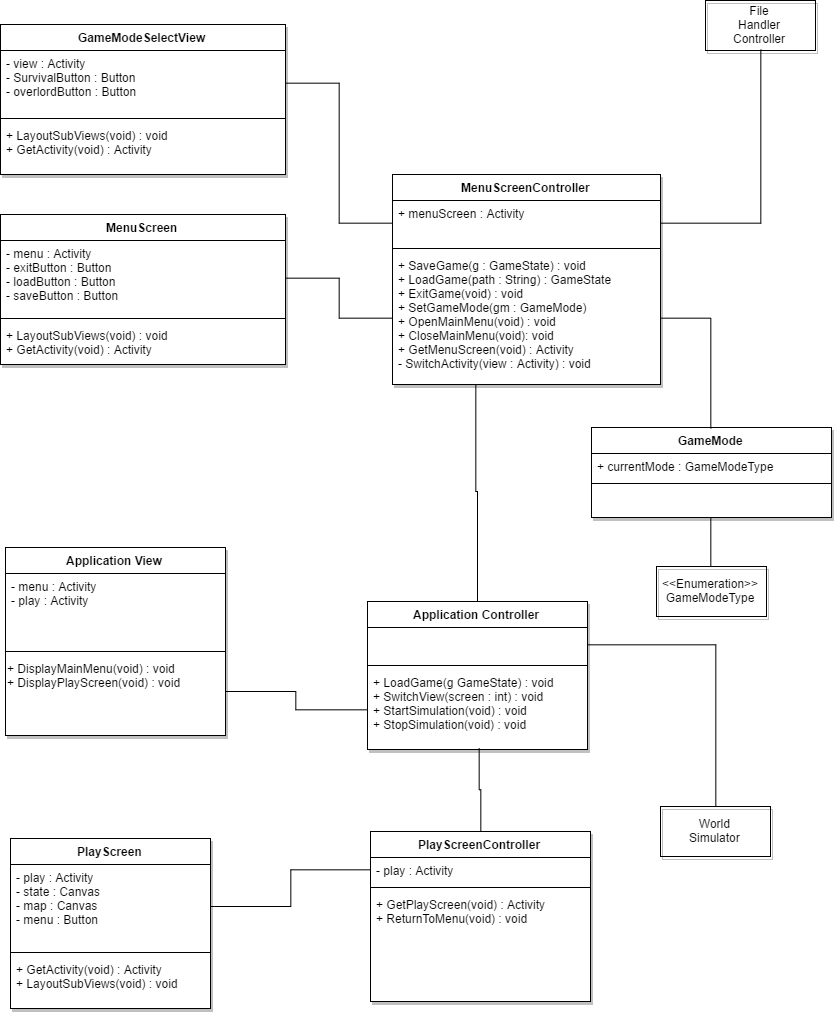
\includegraphics[width=0.8\textwidth , height=15cm, keepaspectratio]{dcdTL}
    \caption{Class Diagram 1/5}
    \label{fig:dcdTL}
\end{figure}

\pagebreak
\begin{figure}[h]
    \centering
    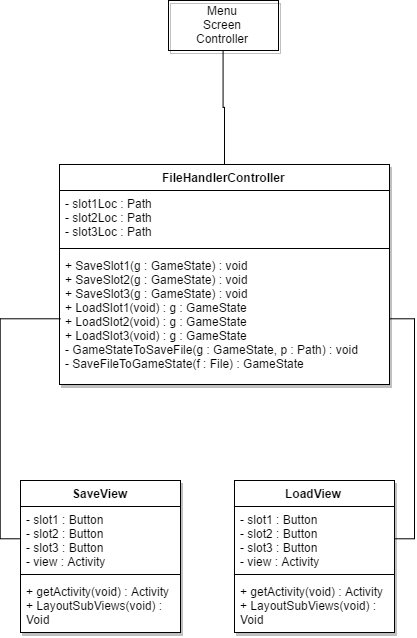
\includegraphics[width=0.8\textwidth , height=12cm, keepaspectratio]{dcdF}
    \caption{Class Diagram 2/5}
    \label{fig:dcdTL}
\end{figure}

\pagebreak
\begin{figure}[h]
    \centering
    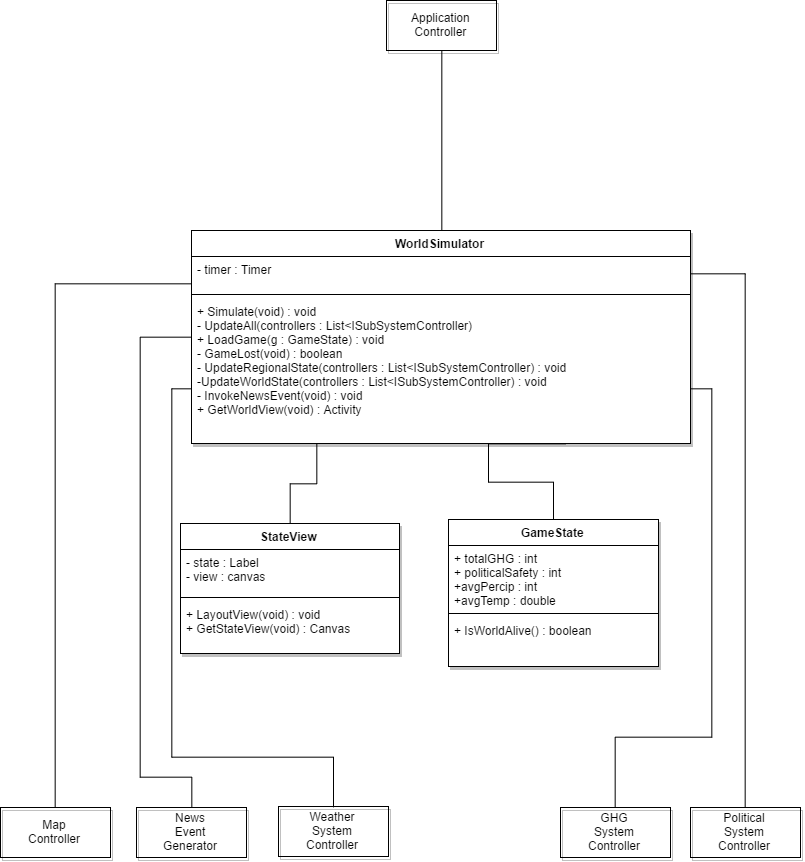
\includegraphics[width=0.8\textwidth , height=15cm, keepaspectratio]{dcdWS}
    \caption{Class Diagram 3/5}
    \label{fig:dcdTL}
\end{figure}

\pagebreak
\begin{figure}[h]
    \centering
    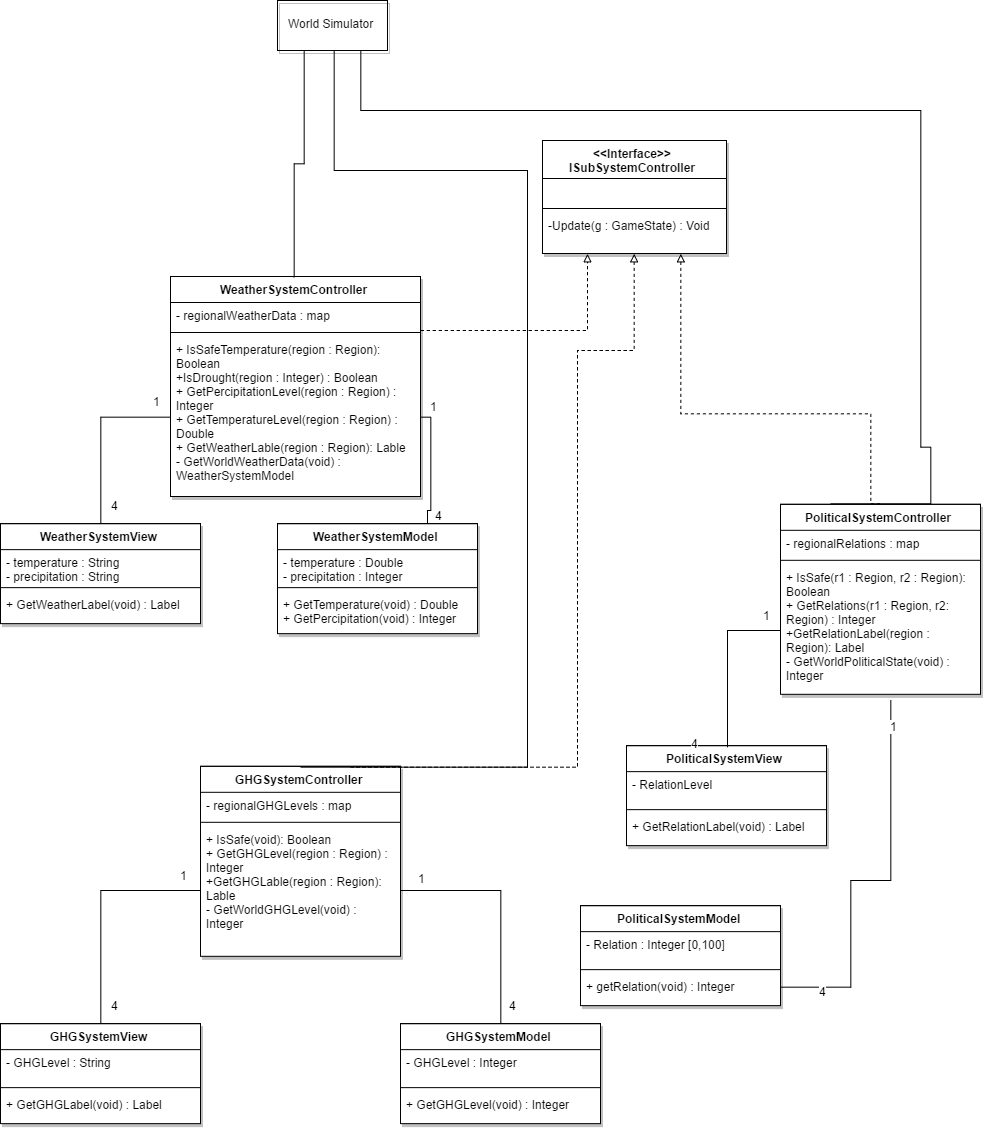
\includegraphics[width=0.8\textwidth , height=15cm, keepaspectratio]{dcdSS}
    \caption{Class Diagram 4/5}
    \label{fig:dcdTL}
\end{figure}

\pagebreak
\begin{figure}[h]
    \centering
    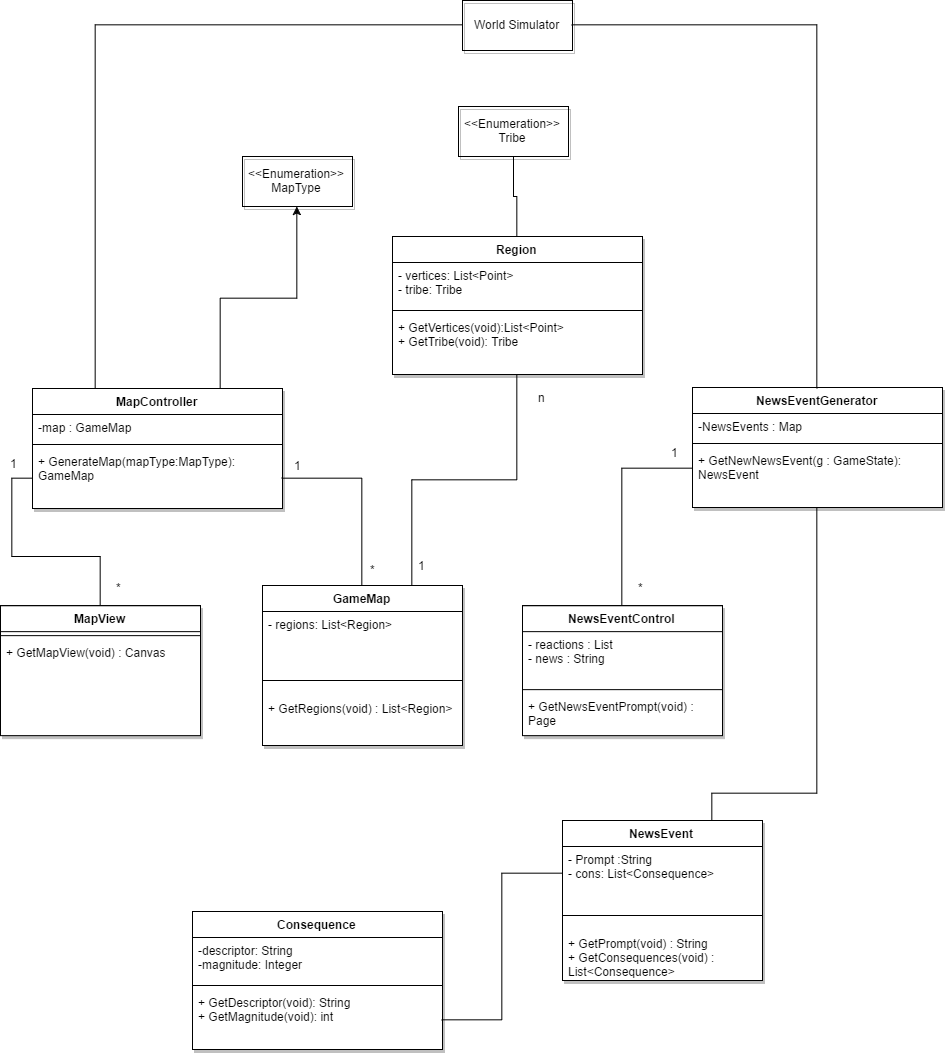
\includegraphics[width=0.8\textwidth , height=15cm, keepaspectratio]{dcdNM}
    \caption{Class Diagram 5/5}
    \label{fig:dcdTL}
\end{figure}

\newpage
% End Section

\appendix
\section{Division of Labour}
\label{sec:division_of_labour}
% Begin Section
Include a Division of Labour sheet which indicates the contributions of each team member. This sheet must be signed by all team members.


\begin{tabular}{ | l | l | }
\hline
	\textbf{Contributor Name} & \textbf{Contributions}  \\
  	\hline
  	Wenbin Yuan &  \\
  	\hline
  	Haris Khan &  \\
  	\hline
		Riley McGee & Draft of Class Diagram, 4.* \\
  	\hline
		Vishesh Gulatee &  \\
  	\hline
		James Taylor & Section 1.* \\
  	\hline
\end{tabular}
\\
\\
By signing below you agree to the work divisions stated above correctly representing all contributions made:


% End Section

\newpage
\section*{IMPORTANT NOTES}
\begin{itemize}
	\item You do \underline{NOT} need to provide a text explanation of each diagram; the diagram should speak for itself
	\item Please document any non-standard notations that you may have used
	\begin{itemize}
		\item \emph{Rule of Thumb}: if you feel there is any doubt surrounding the meaning of your notations, document them
	\end{itemize}
	\item Some diagrams may be difficult to fit into one page
	\begin{itemize}
		\item It is OK if the text is small but please ensure that it is readable when printed
		\item If you need to break a diagram onto multiple pages, please adopt a system of doing so and throughly explain how it can be reconnected from one page to the next; if you are unsure about this, please ask me
	\end{itemize}
	\item Please submit the latest version of Deliverable 1 and Deliverable 2 with Deliverable 3
	\begin{itemize}
		\item They do not have to be a freshly printed versions; the latest marked versions are OK
	\end{itemize}
	\item If you do \underline{NOT} have a Division of Labour sheet, your deliverable will \underline{NOT} be marked
\end{itemize}


\end{document}
%------------------------------------------------------------------------------
